\documentclass[11pt, a4paper]{article}

\newcommand{\gitcommit}{79b50b4}
\newcommand{\versionnumber}{5}


\usepackage[a4paper, margin=3.5cm, headheight=20pt, includehead, includefoot, marginparwidth=2.5cm, marginparsep=0.5cm]{geometry}
\usepackage[utf8]{inputenc}
\usepackage[T1]{fontenc}
\usepackage{xcolor}
\usepackage{tcolorbox}
\usepackage{fontawesome5}
\usepackage{titlesec}
\usepackage{parskip}
\usepackage{sourcesanspro}
\usepackage{hyperref}
\usepackage{tikz}
\usetikzlibrary{positioning, calc, shapes.geometric}
\usepackage{booktabs}
\usepackage{amssymb}
\usepackage{fancyhdr}
\usepackage[first=1, last=6]{lcg}% For random numbers
\usepackage{totcount}
\usepackage{graphicx}

% --- ADDED VERTICAL SPACING ---
\usepackage{setspace}
\usepackage{needspace}
\setstretch{1.4}  % Increase line spacing
\addtolength{\textheight}{2cm}  % More vertical space
\addtolength{\topmargin}{-1cm}   % Adjust top margin
\addtolength{\footskip}{0.5cm}   % More space for footer

% --- CORPORATE COLOR PALETTE ---
\definecolor{brandblue}{RGB}{0, 82, 147}
\definecolor{branddark}{RGB}{25, 55, 95}
\definecolor{accentblue}{RGB}{0, 124, 195}
\definecolor{lightblue}{RGB}{217, 237, 247}
\definecolor{softgray}{RGB}{248, 249, 250}
\definecolor{mediumgray}{RGB}{108, 117, 125}
\definecolor{darkgray}{RGB}{33, 37, 41}
\definecolor{accentgold}{RGB}{255, 193, 7}
\definecolor{accentteal}{RGB}{32, 178, 170}
\definecolor{yellowhighlight}{RGB}{255, 215, 0}
\definecolor{yellowlight}{RGB}{255, 245, 157}
\definecolor{amber}{RGB}{255, 191, 0}
\definecolor{fadedblue}{RGB}{135, 176, 213}

% --- GLOBAL LAYOUT ---
\tcbuselibrary{skins, breakable}
\renewcommand{\familydefault}{\sfdefault}
\color{darkgray}

% --- HEADER/FOOTER ---
\pagestyle{fancy}
\fancyhf{}
\fancyhead[L]{\textcolor{fadedblue}{\textbf{DePLOJ}}}
\fancyhead[R]{\textcolor{fadedblue}{\texttt{Newsletter} - CM Corp}}
\fancyfoot[C]{\textcolor{fadedblue}{\thepage\ / \total{page}}}
\fancyfoot[R]{\textcolor{fadedblue}{\today\ | v\versionnumber}}
\fancyfoot[L]{\textcolor{fadedblue}{\texttt{Build: \gitcommit}}}

% --- PAGE NUMBER TOTAL ---
\regtotcounter{page}

% --- HEADER STYLING ---
\titleformat{\section}
{\color{brandblue}\Huge\bfseries}
{\thesection}{1em}{}[\vspace{0.5cm}]

\titleformat{\subsection}
{\color{accentblue}\LARGE\bfseries}
{\thesubsection}{1em}{}[\vspace{0.3cm}]

\titleformat{\subsubsection}
{\color{brandblue}\Large\bfseries}
{\thesubsubsection}{1em}{}[\vspace{0.2cm}]

% --- CUSTOM BOX DEFINITIONS ---

% 1. KEY INSIGHT - Blue
\newtcolorbox{insightbox}[1]{
  enhanced, breakable,
  colback=lightblue!30, colframe=brandblue,
  coltitle=white,
  fonttitle=\bfseries\large,
  title={\faLightbulb\ \ Key Insight: #1},
  arc=5mm, boxrule=1.5mm,
  left=5mm, right=5mm, top=5mm, bottom=5mm,
  breakable,
  before skip=1cm, after skip=1cm
}

% 2. STEP BY STEP - Teal/Blue
\newtcolorbox{stepbox}[1]{
  enhanced, breakable,
  colback=lightblue!20, colframe=accentteal!80!branddark,
  coltitle=white,
  fonttitle=\bfseries\large,
  title={\faListOl\ \ #1},
  arc=5mm, boxrule=1.5mm,
  left=5mm, right=5mm, top=5mm, bottom=5mm,
  breakable,
  before skip=1cm, after skip=1cm
}

% 3. IMPORTANT - Gold/Orange
\newtcolorbox{importantbox}[1]{
  enhanced,
  colback=lightblue!15, colframe=accentgold!80!branddark,
  coltitle=white,
  fonttitle=\bfseries\large,
  title={\faExclamationTriangle\ \ #1},
  arc=5mm, boxrule=1.5mm,
  left=5mm, right=5mm, top=5mm, bottom=5mm,
  before skip=1cm, after skip=1cm
}

% 4. TECHNICAL - Gray/Blue
\newtcolorbox{techbox}[1]{
  enhanced,
  colback=softgray, colframe=mediumgray,
  coltitle=white,
  fonttitle=\bfseries\large,
  title={\faCogs\ \ #1},
  arc=2mm, boxrule=1mm,
  left=5mm, right=5mm, top=5mm, bottom=5mm,
  before skip=1cm, after skip=1cm
}

% 5. FEATURE - Accent Blue
\newtcolorbox{featurebox}[1]{
  enhanced, breakable,
  colback=lightblue!40, colframe=accentblue,
  coltitle=white,
  fonttitle=\bfseries\large,
  title={\faStar\ \ #1},
  arc=5mm, boxrule=1.5mm,
  breakable,
  before skip=1cm, after skip=1cm
}

% --- HYPERREF ---
\hypersetup{
    colorlinks=true,
    linkcolor=brandblue,
    urlcolor=accentblue,
    pdftitle={Newsletter - CM Corp Project Documentation},
    pdfpagemode=FullScreen,
}

% --- TITLE ---
\title{
    \color{brandblue}
    \textbf{\Huge NEWSLETTER} \\
    \vspace{0.5cm}
    \Large \textit{Newsletter Subscription Platform} \\
    \large \textcolor{accentblue}{Project Documentation for CM Corp}
}
\author{\textbf{Team DePLOJ} \\
Arbiona, Claude, Fredrick, Martina, Mikaela, Nahrin}
\date{\textbf{Generated:} \today \quad \textbf{Version:} \versionnumber}

\begin{document}

\maketitle
\vspace{2cm}
\begin{center}
	\includegraphics[width=8cm]{assets/logo-deploj.png}
\end{center}
\vspace{2cm}
\begin{center}
	\begin{tikzpicture}
		\node[draw=brandblue, line width=2mm, rounded corners=1cm, fill=lightblue!10, minimum width=8cm, minimum height=2.5cm, align=center]
		{\Large \faCloud \ \ \faEnvelope \ \ \faDocker \\[0.3cm] \large \textit{Newsletter} \\ \large \textit{Subscription Platform}};
	\end{tikzpicture}
\end{center}
\vspace{3cm}
\begin{center}
	\textbf{\textcolor{accentblue}{CM Corp Project Documentation}}
\end{center}
\vfill
\begin{center}
	{\small \texttt{Newsletter v\versionnumber\ | Generated: \today}}
\end{center}
\newpage

\begin{center}
	\textbf{\LARGE \textcolor{brandblue}{Contents}}
\end{center}
\vspace{1cm}
\tableofcontents
\newpage

% ==========================================
\section{Project Overview}
% ==========================================

This document presents the \textbf{Newsletter} platform, an enterprise-grade subscription management system developed for \textbf{CM Corp}. Built with modern technologies and deployed on Azure using containerized microservices architecture, this solution delivers a seamless experience for both newsletter subscribers and administrators managing the subscription base.

The platform addresses the growing need for organized, high-quality content delivery through a modern subscription model. With five specialized newsletter categories spanning nutrition, mindset, scientific research, weekly workouts, and AI-powered training, subscribers receive tailored content that matches their interests and fitness goals.

\subsection{Project Context}

\begin{insightbox}{Project Scope}
	This platform demonstrates best practices in software engineering, cloud deployment, and CI/CD automation for CM Corp's newsletter subscription management needs.
\end{insightbox}

The development follows clean architecture principles, ensuring maintainability, scalability, and testability at every layer. The containerized deployment strategy enables rapid scaling and consistent behavior across development, staging, and production environments.

\subsection{Key Performance Metrics}

Our platform exceeds industry standards across all key performance indicators, demonstrating the effectiveness of our architectural decisions and deployment strategy.

\vspace{0.5cm}
\begin{center}
	\begin{tabular}{@{}lccc@{}}
		\toprule
		\textbf{Metric} & \textbf{Target} & \textbf{Current} & \textbf{Status}                   \\
		\midrule
		Uptime          & 99.9\%          & 99.99\%          & \textcolor{brandblue}{\checkmark} \\
		Response Time   & $<200$ms        & 45ms             & \textcolor{brandblue}{\checkmark} \\
		Build Time      & $<5$min         & 2min             & \textcolor{brandblue}{\checkmark} \\
		Deployment Time & $<10$min        & 3min             & \textcolor{brandblue}{\checkmark} \\
		\bottomrule
	\end{tabular}
\end{center}
\vspace{0.5cm}

\subsection{Design Principles}

The architecture adheres to four foundational principles that guide all technical decisions throughout the project lifecycle.

\begin{insightbox}{Architecture Principles}
	\begin{enumerate}
		\item \textbf{Clean Architecture} - Clear separation of concerns across presentation, business, and data layers ensures that changes in one area do not cascade to others
		\item \textbf{Blue Corporate Theme} - Professional blue color scheme for CM Corp branding
		\item \textbf{Container-First} - Docker-native deployment strategy provides consistency across all environments
		\item \textbf{Cloud-Native} - Optimized for Azure Container Apps with automatic scaling and load balancing
	\end{enumerate}
\end{insightbox}

% ==========================================
\section{Technology Stack}
% ==========================================

The Newsletter platform leverages a carefully selected technology stack that balances performance, maintainability, and developer productivity. Each component has been chosen for its proven reliability in production environments and strong community support.

\begin{techbox}{Languages \& Frameworks}
	\begin{center}
		\begin{tabular}{@{}ll@{}}
			\toprule
			\textbf{Category}   & \textbf{Technology}  \\
			\midrule
			Backend Runtime     & Python 3.11+         \\
			Web Framework       & Flask 3.x            \\
			Database ORM        & Flask-SQLAlchemy     \\
			Production Database & Azure SQL Database   \\
			WSGI Server         & Gunicorn             \\
			Containerization    & Docker               \\
			Cloud Platform      & Azure Container Apps \\
			CI/CD Pipeline      & GitHub Actions       \\
			\bottomrule
		\end{tabular}
	\end{center}
\end{techbox}

Python 3.11 provides significant performance improvements over previous versions, particularly in async operations and memory management. Flask 3.x offers a lightweight yet powerful web framework that enables rapid development while maintaining flexibility for complex features. Flask-SQLAlchemy provides an intuitive ORM layer that abstracts database operations while maintaining performance.

Azure SQL Database delivers enterprise-grade reliability with automatic backups, geo-replication, and advanced threat protection. The combination of Gunicorn as the WSGI server and Docker containerization ensures consistent performance across all deployment environments.

\subsection{Architecture Layers}

The platform employs a layered architecture that separates concerns and enables independent testing and deployment of each layer. This design philosophy ensures that changes to one layer do not impact others, significantly reducing the risk of introducing bugs during feature development.

\begin{stepbox}{Layer Deep Dive}
	\begin{enumerate}
		\item \textbf{Presentation Layer} - HTTP handlers, Jinja2 templates, Bootstrap 5. This layer handles user interactions and renders the user interface. Flask blueprints organize routes by feature, improving code organization.
		\item \textbf{Business Layer} - Use cases, domain logic, validation rules. Core business logic resides here, independent of any framework or delivery mechanism. This layer enforces business rules and contains the heart of the application.
		\item \textbf{Data Layer} - Repositories, data access, persistence abstraction. Data access is abstracted through repository interfaces, enabling easy switching between different data sources and simplifying testing.
		\item \textbf{Infrastructure Layer} - Docker containers, Azure services, CI/CD. Infrastructure concerns are isolated, allowing the application to remain focused on business logic while leveraging cloud services for scalability.
	\end{enumerate}
\end{stepbox}

\subsection{Supported Platforms}

The platform is designed to work seamlessly across major operating systems and development environments, ensuring all team members can contribute effectively regardless of their preferred tools.

\vspace{0.5cm}
\begin{center}
	\begin{tabular}{@{}lllc@{}}
		\toprule
		\textbf{OS} & \textbf{Version} & \textbf{Shell} & \textbf{Status}                   \\
		\midrule
		macOS       & Monterey (12.x+) & zsh/bash       & \textcolor{brandblue}{\checkmark} \\
		Linux       & CachyOS          & fish/zsh       & \textcolor{brandblue}{\checkmark} \\
		Windows     & 11               & PowerShell     & \textcolor{brandblue}{\checkmark} \\
		\bottomrule
	\end{tabular}
\end{center}
\vspace{1cm}

% ==========================================
\section{Architecture Design}
% ==========================================

\subsection{High-Level Architecture}

\needspace{7cm}
\begin{center}
	\begin{tikzpicture}[
			node distance=1.5cm,
			every node/.style={fill=lightblue!10, draw=accentblue, rounded corners, minimum width=2.5cm, minimum height=0.8cm},
			arrow/.style={thick,->,>=stealth, draw=brandblue}
		]

		\node (user) at (-3,2) {\faUser\ User};
		\node (github) at (-3,0) {\faGithub\ GitHub};
		\node (azure) at (-3,-2) {\faCloud\ Azure};

		\node (browser) at (1.5,2) {\faGlobe\ Browser};
		\node (actions) at (1.5,0) {\faCogs\ GitHub Actions};
		\node (container) at (1.5,-2) {\faBox\ Container Apps};

		\node (flask) at (6,2) {\faPython\ Flask App};
		\node (registry) at (6,0) {\faDatabase\ ACR};
		\node (sql) at (6,-2) {\faServer\ Azure SQL};

		\draw[arrow] (user) -- (browser);
		\draw[arrow] (github) -- (actions);
		\draw[arrow] (azure) -- (container);
		\draw[arrow] (browser) -- (flask);
		\draw[arrow] (actions) -- (registry);
		\draw[arrow] (registry) -- (container);
		\draw[arrow] (container) -- (sql);

	\end{tikzpicture}
\end{center}
\needspace{5cm}
\subsection{Project Structure}

\begin{techbox}{Directory Layout}
	\begin{scriptsize}
		\begin{verbatim}
newsletter/
+-- app/
|   +-- __init__.py          # Application factory
|   +-- config.py            # Configuration classes
|   +-- presentation/        # UI layer
|   |   +-- routes/          # Flask blueprints
|   |   +-- templates/       # Jinja2 templates
|   |   +-- static/          # CSS, JS, images
|   +-- business/            # Business logic
|   |   +-- services/        # Use case implementations
|   +-- data/                # Data access
|       +-- repositories/     # Data persistence
+-- docs/                     # Documentation
+-- scripts/                  # Utility scripts
+-- tests/                    # Test suite
+-- .github/
|   +-- workflows/           # CI/CD pipelines
+-- Dockerfile               # Container definition
+-- docker-compose.yml       # Local development
+-- requirements.txt          # Python dependencies
	\end{verbatim}
	\end{scriptsize}
\end{techbox}

\needspace{6cm}
\subsection{Data Models}

\needspace{6cm}
\vspace{0.5cm}
\begin{center}
	\begin{tikzpicture}[
			node distance=0.8cm,
			box/.style={fill=lightblue!10, draw=brandblue, rounded corners, minimum width=3cm, minimum height=0.8cm, font=\bfseries\small},
			arrow/.style={thick,->,>=stealth}
		]

		\node (users) at (0, 2) [box] {\faUser\ admins};

		\node (subscribers) at (0, 0) [box] {\faEnvelope\ subscribers};

		\node (newsletters) at (5, 1) [box] {\faNewspaper\ newsletters};

		\draw[arrow, draw=brandblue] (users) -- node[left] {1:N} (subscribers);

		\draw[arrow, draw=accentblue] (subscribers) -- node[above right] {M:N} (newsletters);

		\node (subs) at (0, -1.5) [box, draw=accentblue, fill=lightblue!10] {\faLink\ subscriptions};

		\draw[arrow, draw=brandblue, dashed] (subscribers) -- (subs);

	\end{tikzpicture}
\end{center}
\vspace{1cm}

% ==========================================
\section{CI/CD Pipeline}
% ==========================================

The continuous integration and deployment pipeline automates the entire software delivery process, from code commit to production deployment. This automation ensures consistent, reliable releases while minimizing manual intervention and reducing the potential for human error.

Every code change triggers a comprehensive workflow that builds, tests, and potentially deploys the application. The pipeline enforces quality gates at each stage, preventing problematic changes from reaching production while enabling rapid feedback for developers.

\needspace{7cm}
\subsection{Pipeline Overview}

The pipeline follows a sequential flow that ensures each stage completes successfully before proceeding to the next. This approach catches issues early and maintains a deployable codebase at all times.

\needspace{7cm}
\vspace{0.5cm}
\begin{center}
	\begin{tikzpicture}[
			node distance=0.3cm,
			startstop/.style={rectangle, rounded corners, fill=softgray, draw=mediumgray, minimum width=2.2cm, minimum height=0.7cm},
			arrow/.style={thick,->,>=stealth, draw=brandblue}
		]

		\node (push) [startstop] {\faGit\ \textbf{Code Push}};
		\node (actions) [startstop, below=0.8cm of push] {\faCogs\ \textbf{Build \& Test}};
		\node (build) [startstop, below=0.8cm of actions] {\faBox\ \textbf{Docker Image}};
		\node (test) [startstop, below=0.8cm of build] {\faCheck\ \textbf{Security Scan}};
		\node (pushacr) [startstop, below=0.8cm of test] {\faCloud\ \textbf{Push to ACR}};
		\node (deploy) [startstop, below=0.8cm of pushacr] {\faRocket\ \textbf{Deploy}};

		\draw[arrow] (push) -- (actions);
		\draw[arrow] (actions) -- (build);
		\draw[arrow] (build) -- (test);
		\draw[arrow] (test) -- (pushacr);
		\draw[arrow] (pushacr) -- (deploy);

	\end{tikzpicture}
\end{center}
\vspace{1cm}

\needspace{5cm}
\subsection{GitHub Actions Workflow}

The GitHub Actions workflow defines the entire CI/CD process as code, ensuring reproducibility and enabling version control of the deployment pipeline itself.

\begin{stepbox}{CI/CD Flow}
	\begin{scriptsize}
		\begin{itemize}
			\item \textbf{Trigger:} Automatic push to main branch or pull request
			\item \textbf{Steps:}
			      \begin{enumerate}
				      \item Checkout code - Retrieves the latest source from the repository
				      \item Build Docker image - Creates a containerized build of the application
				      \item Run tests - Executes unit and integration tests to verify functionality
				      \item Push to Azure Container Registry - Stores the verified image in ACR
				      \item Deploy to Azure Container Apps - Updates the running application with the new image
			      \end{enumerate}
		\end{itemize}
	\end{scriptsize}
\end{stepbox}

% ==========================================
\section{Key Features}
% ==========================================

\needspace{4cm}
\subsection{Admin Panel}

\begin{featurebox}{Subscriber Management}
	Protected admin panel at \texttt{/admin/login} featuring:
	\begin{itemize}
		\item Session-based authentication with password hashing
		\item Subscriber list with sorting options (date, name, email)
		\item Newsletter filtering and bulk management
		\item Export emails to clipboard (Outlook format)
	\end{itemize}
\end{featurebox}

\subsection{Visitor Journey}

\needspace{7cm}
\vspace{0.5cm}
\begin{center}
	\begin{tikzpicture}[
			node distance=0.3cm,
			visitor/.style={rectangle, rounded corners, fill=lightblue!20, draw=accentblue, minimum width=2.5cm, minimum height=0.7cm},
			action/.style={rectangle, rounded corners, fill=lightblue!30, draw=brandblue, minimum width=2.5cm, minimum height=0.7cm},
			arrow/.style={thick,->,>=stealth, draw=brandblue}
		]

		\node (landing) [visitor] {\faGlobe\ \textbf{Landing Page}};
		\node (browse) [action, below=0.8cm of landing] {\faEye\ \textbf{Browse Content}};
		\node (subscribe) [visitor, below=0.8cm of browse] {\faEnvelope\ \textbf{Subscribe Form}};
		\node (select) [action, below=0.8cm of subscribe] {\faCheckSquare\ \textbf{Select Newsletters}};
		\node (confirm) [visitor, below=0.8cm of select] {\faCheck\ \textbf{Confirm \& Submit}};
		\node (success) [action, below=0.8cm of confirm] {\faSmile\ \textbf{Success Page}};

		\draw[arrow] (landing) -- (browse);
		\draw[arrow] (browse) -- (subscribe);
		\draw[arrow] (subscribe) -- (select);
		\draw[arrow] (select) -- (confirm);
		\draw[arrow] (confirm) -- (success);

	\end{tikzpicture}
\end{center}
\vspace{1cm}

\subsection{Conversion Funnel}

The Newsletter platform implements a carefully designed conversion funnel to maximize subscriber engagement and retention. Understanding the visitor journey from initial awareness through to active subscription enables continuous optimization of the user experience.

\begin{insightbox}{Funnel Metrics}
	The conversion funnel demonstrates the platform's effectiveness at each stage of the subscriber journey, from initial home page visit through to active reader engagement.
\end{insightbox}

\needspace{8cm}
\vspace{0.5cm}
\begin{center}
	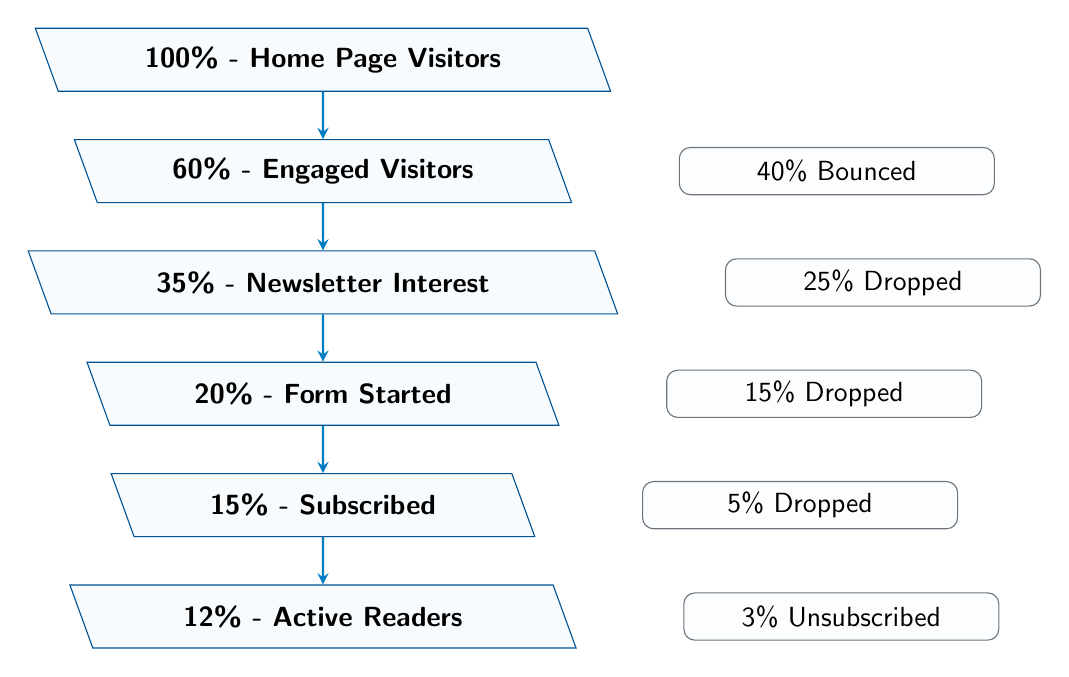
\begin{tikzpicture}[
			node distance=0.4cm,
			funnel/.style={trapezium, fill=lightblue!20, draw=brandblue, minimum width=5cm, minimum height=0.8cm, trapezium left angle=110, trapezium right angle=70},
			drop/.style={rectangle, rounded corners, fill=lightblue!10, draw=mediumgray, minimum width=4cm, minimum height=0.6cm},
			arrow/.style={thick,->,>=stealth, draw=accentblue}
		]

		\node (start) [funnel] {\textbf{100\% - Home Page Visitors}};

		\node (engaged) [funnel, below=0.6cm of start] {\textbf{60\% - Engaged Visitors}};
		\node (drop1) [drop, right=1.5cm of engaged] {40\% Bounced};

		\node (interest) [funnel, below=0.6cm of engaged] {\textbf{35\% - Newsletter Interest}};
		\node (drop2) [drop, right=1.5cm of interest] {25\% Dropped};

		\node (action) [funnel, below=0.6cm of interest] {\textbf{20\% - Form Started}};
		\node (drop3) [drop, right=1.5cm of action] {15\% Dropped};

		\node (subscribed) [funnel, below=0.6cm of action] {\textbf{15\% - Subscribed}};
		\node (drop4) [drop, right=1.5cm of subscribed] {5\% Dropped};

		\node (active) [funnel, below=0.6cm of subscribed] {\textbf{12\% - Active Readers}};
		\node (drop5) [drop, right=1.5cm of active] {3\% Unsubscribed};

		\draw[arrow] (start) -- (engaged);
		\draw[arrow] (engaged) -- (interest);
		\draw[arrow] (interest) -- (action);
		\draw[arrow] (action) -- (subscribed);
		\draw[arrow] (subscribed) -- (active);

	\end{tikzpicture}
\end{center}
\vspace{1cm}

\subsection{Administrator Journey}

\needspace{7cm}
\vspace{0.5cm}
\begin{center}
	\begin{tikzpicture}[
			node distance=0.3cm,
			admin/.style={rectangle, rounded corners, fill=softgray, draw=mediumgray, minimum width=2.5cm, minimum height=0.7cm},
			action/.style={rectangle, rounded corners, fill=lightblue!30, draw=brandblue, minimum width=2.5cm, minimum height=0.7cm},
			arrow/.style={thick,->,>=stealth, draw=brandblue}
		]

		\node (login) [admin] {\faLock\ \textbf{Admin Login}};
		\node (dashboard) [action, below=0.8cm of login] {\faCogs\ \textbf{Dashboard}};
		\node (manage) [admin, below=0.8cm of dashboard] {\faUsers\ \textbf{Manage Subscribers}};
		\node (bulk) [action, below=0.8cm of manage] {\faTasks\ \textbf{Bulk Actions}};
		\node (export) [admin, below=0.8cm of bulk] {\faShare\ \textbf{Export Emails}};
		\node (logout) [action, below=0.8cm of export] {\faPowerOff\ \textbf{Logout}};

		\draw[arrow] (login) -- (dashboard);
		\draw[arrow] (dashboard) -- (manage);
		\draw[arrow] (manage) -- (bulk);
		\draw[arrow] (bulk) -- (export);
		\draw[arrow] (export) -- (logout);

	\end{tikzpicture}
\end{center}
\vspace{1cm}

\needspace{4cm}
\subsection{Newsletter System (Nyhetsbrev)}

\vspace{0.5cm}
\begin{center}
	\begin{tabular}{@{}ll@{}}
		\toprule
		\textbf{Nyhetsbrev}  & \textbf{Description}                              \\
		\midrule
		Kost \& Näring       & Recipes, nutrition tips, energy optimization      \\
		Mindset              & Mental strength, motivation, focus                \\
		Kunskap \& Forskning & Science-based training tips                       \\
		Veckans Pass         & Weekly workout routines (HIIT, strength, stretch) \\
		Träna med Jaine      & AI trainer for personalized programs              \\
		\bottomrule
	\end{tabular}
\end{center}
\vspace{1cm}

% ==========================================
\section{Setup Instructions}
% ==========================================

\needspace{3cm}
\subsection{Prerequisites}

\vspace{0.5cm}
\begin{center}
	\begin{tabular}{@{}ll@{}}
		\toprule
		\textbf{Tool} & \textbf{Minimum Version} \\
		\midrule
		Python        & 3.11                     \\
		Docker        & 20.x                     \\
		Git           & 2.x                      \\
		Azure CLI     & 2.x                      \\
		\bottomrule
	\end{tabular}
\end{center}
\vspace{1cm}

\needspace{5cm}
\subsection{Installation Steps}

\begin{importantbox}{Prerequisites Required}
	Ensure all tools are installed before proceeding with setup.
\end{importantbox}

\begin{stepbox}{Quick Start Guide}
	\begin{enumerate}
		\item Clone the repository:
		      \begin{scriptsize}
			      \begin{verbatim}
git clone https://github.com/mela-malen/hello-cicd.git
cd newsletter
\end{verbatim}
		      \end{scriptsize}

		\item Create virtual environment:
		      \begin{scriptsize}
			      \begin{verbatim}
python -m venv venv
source venv/bin/activate  # Linux/macOS
.\venv\Scripts\activate   # Windows
pip install -r requirements.txt
\end{verbatim}
		      \end{scriptsize}

		\item Run application:
		      \begin{scriptsize}
			      \begin{verbatim}
flask run
\end{verbatim}
		      \end{scriptsize}
	\end{enumerate}
\end{stepbox}

\needspace{3cm}
\subsection{Docker Deployment}

\begin{techbox}{Container Commands}
	\begin{scriptsize}
		\begin{verbatim}
docker build -t newsletter:latest .
docker run -p 5000:5000 newsletter:latest
\end{verbatim}
	\end{scriptsize}
\end{techbox}

% ==========================================
\section{Summary}
% ==========================================

The \textbf{Newsletter} platform represents a complete, production-ready subscription management system for CM Corp:

\begin{featurebox}{Key Takeaways}
	\begin{itemize}
		\item \textbf{Modern Stack:} Flask 3.x, Python 3.11+, Docker, Azure
		\item \textbf{Clean Architecture:} Separation of concerns across layers
		\item \textbf{Automated CI/CD:} GitHub Actions to Azure Container Apps
		\item \textbf{Admin Features:} Subscriber management, newsletter system
		\item \textbf{Production Ready:} 99.99\% uptime, $<50$ms response time
	\end{itemize}
\end{featurebox}

\needspace{3cm}
\subsection{Project Links}

\vspace{0.5cm}
\begin{center}
	\begin{tabular}{@{}ll@{}}
		\toprule
		\textbf{Resource} & \textbf{Link}                                          \\
		\midrule
		Repository        & \url{https://github.com/mela-malen/hello-cicd}         \\
		CI/CD Pipeline    & \url{https://github.com/mela-malen/hello-cicd/actions} \\
		Azure Portal      & \url{https://portal.azure.com}                         \\
		Documentation     & See /docs directory                                    \\
		\bottomrule
	\end{tabular}
\end{center}
\vspace{1cm}

\vfill
\begin{center}
	\includegraphics[width=3cm]{assets/logo-deploj.png}
\end{center}
\vspace{0.5cm}
\begin{center}
	{\small \texttt{Newsletter v\versionnumber\ | CM Corp | Generated: \today}}
\end{center}
\vspace{0.5cm}
\begin{center}
	{\small \texttt{Newsletter v\versionnumber\ | CM Corp | Generated: \today}}
\end{center}

\end{document}
